\documentclass[12pt]{article}
\usepackage[margin=1in]{geometry}
\usepackage[utf8]{inputenc}
\usepackage{datetime}
\usepackage{caption}
\usepackage{cite}
\usepackage[hyphens]{url}
\usepackage[numbers]{natbib}
\usepackage[table, dvipsnames]{xcolor}
\usepackage{lscape}
\usepackage{tikz}
\usetikzlibrary{arrows}

\newdateformat{monthyeardate}{\monthname[\THEMONTH], \THEYEAR}

\newcommand{\todo}[1]{{\color{red}[\textbf{TODO:} #1]}}
\renewcommand*{\bibfont}{\raggedright}

\title{History of Project Teams at Cornell}
\author{Alex Renda (adr74)}
\date{\monthyeardate\today}

\begin{document}

\maketitle

\section{Introduction}

Project teams are a core part of the College of Engineering at Cornell.
These groups have disparate goals, from building racecars and bridges to designing phone apps for social good, but one commonality links them all: they are entirely student-led and student-run, and they provide a home for students across Cornell, both within engineering and outside of it.
In 2015, Kate Klein noted that ``a quarter of all undergraduate engineering students participate on a growing number of project teams''~\cite{klein_engineering_2015}.
This number has only grown since then:
``as of 2018, there are 29 different project teams, with over 1,100 students and over \$1,000,000 in funding''~\cite{noauthor_project_2018}.
With 3,116 undergraduate students in engineering~\cite{westervelt_key_2017}, over a third of engineering students are currently on project teams, higher than the percentage of Cornell students in Greek life~\cite{noauthor_sorority_2017}.
Despite these impressive numbers, there is relatively little literature on the history and current status of engineering project teams at Cornell.
As of the time of writing this report, the endowed position of project team director is vacant, and there is nearly no official university information about the new lab space for teams, or nearly of the many project teams formed in the past several years.

In this report, I will attempt to remedy some of that lack of information.
In Section~\ref{sec:background}, I will detail the background of project teams at Cornell, including the origins of some of the oldest project teams at Cornell, along with the creation of project teams as an official program at Cornell.
In Section~\ref{sec:timeline}, I will discuss the general timeline of project teams at Cornell, including the explosion in popularity in recent years.
Finally, in Section~\ref{sec:cuauv}, I will delve into the history of a specific project team, the Cornell University Autonomous Underwater Vehicle team (CUAUV), to explore how rich the history is for just one of Cornell's 29 thriving student-led project teams.

\section{Institutional Background}
\label{sec:background}
While practical projects have been a part of engineering curricula since time immemorial, it has only been in the past 30 or so years that student-run teams to compete in extracurricular challenges or solve societal problems have come into their own at Cornell.

According the Rebecca Macdonald, the former Swanson Director of Engineering Student Project Teams, ``Cornell Racing is the `granddaddy' of engineering project teams''~\cite{klein_engineering_2015}. Cornell Racing was formed in 1986~\cite{noauthor_cornell_2012} to compete in Formula SAE, a competition inaugurated in 1981 in which students design and build a racecar to compete in a Formula One style race~\cite{sae_international_formula_2018}.

Cornell Racing's development mirrors that of both of the other three oldest project teams: both Steel Bridge and ACM Programming were formed as student groups competing in inter-university competitions (respectively the Student Chapters of the American Society of Civil Engineers' bridge-building contest~\cite{robert_e._shaw_jr._bridging_1988}, and the Association for Computing Machinery's International Collegiate Programming Contest~\cite{poucher_early_2011}).

While the early project teams thrived on their own, often taking top places in their competitions~\cite{noauthor_cuauv_2003}, it wasn't until 2012 that project teams took on a more official role at Cornell, when a \$5 million dollar gift endowed both the project teams themselves, as well as the full-time position of the Swanson Director of Engineering Student Project Teams~\cite{emily_hopkins_10_2012}.
This gift led to the hiring of a full-time director of project teams, Rebecca Macdonald, to supplant the part-time support that had been previously given by Matt Ulinsky~\cite{thomas_putting_2013}.

Along with Rebecca Macdonald's tenure came a renovation of Upson Hall, with a focus on increased resources for project teams.
According to a College of Engineering document on Upson Hall, ``the renovation will increase the size of Cornell Engineering student team's Experiential Learning Lab in the lower level of Upson Hall by 50\%.''~\cite{noauthor_cornell_2015-1}.
The renovation was completed and project teams moved in during August 2017, providing a significantly larger and more modern space than the project teams had enjoyed in the last several years.

Unfortunately, although Rebecca Macdonald was in large part responsible for the creation of the project team space during the Upson renovation~\cite{noauthor_q&rebecca_2014}, she departed during the summer of 2017~\cite{macdonald_thank_2017}, and was temporarily replaced by Mike Thompson~\cite{ivory_thank_2017} pending appointment of another Swanson Director of Engineering Student Project Teams.

Through this all, project teams have become more and more relevant on campus, even outside of their immediate membership.
There is probably no better place to see this than in the unofficial courses that some project teams have started teaching.
For instance, as of 2017, ``The Cornell Data Science project team will launch an unofficial student-led training course this semester — taught and developed entirely by Cornell students — to help students gain hands-on experience in the increasingly valuable skills of statistical methods and programming languages.''~\cite{si_cornell_2017}.
Similar 2-credit courses are also offered by Cornell AppDev~\cite{noauthor_cornell_2018-5}, impacting people outside of just the engineering department or the people on the project teams.

\section{Timeline}
\label{sec:timeline}

As discussed in Section~\ref{sec:background}, the oldest project teams at Cornell date back 20-30 years.
Most, however, follow a more Zipfian distribution, with over two thirds of them having been started in the last 10 years, and nearly half being started in the last 5.
``We registered Hyperloop as a project team because that was the best way to get resources and support from Cornell for our project'' said Alana Marzoev (a founding team lead of the Cornell Hyperloop project team) when asked about why she helped form Cornell Hyperloop as a project team rather than just the club that it was before~\cite{marzoev_rationale_2018}.

These overall trends can be explained by a number of factors.
Most importantly is simply money: 2012 saw an official endowment and source of university funding for project teams, meaning that there is more incentive and rationale to create a project team.
The explosion %
\begin{landscape} %
  \begin{figure} %
    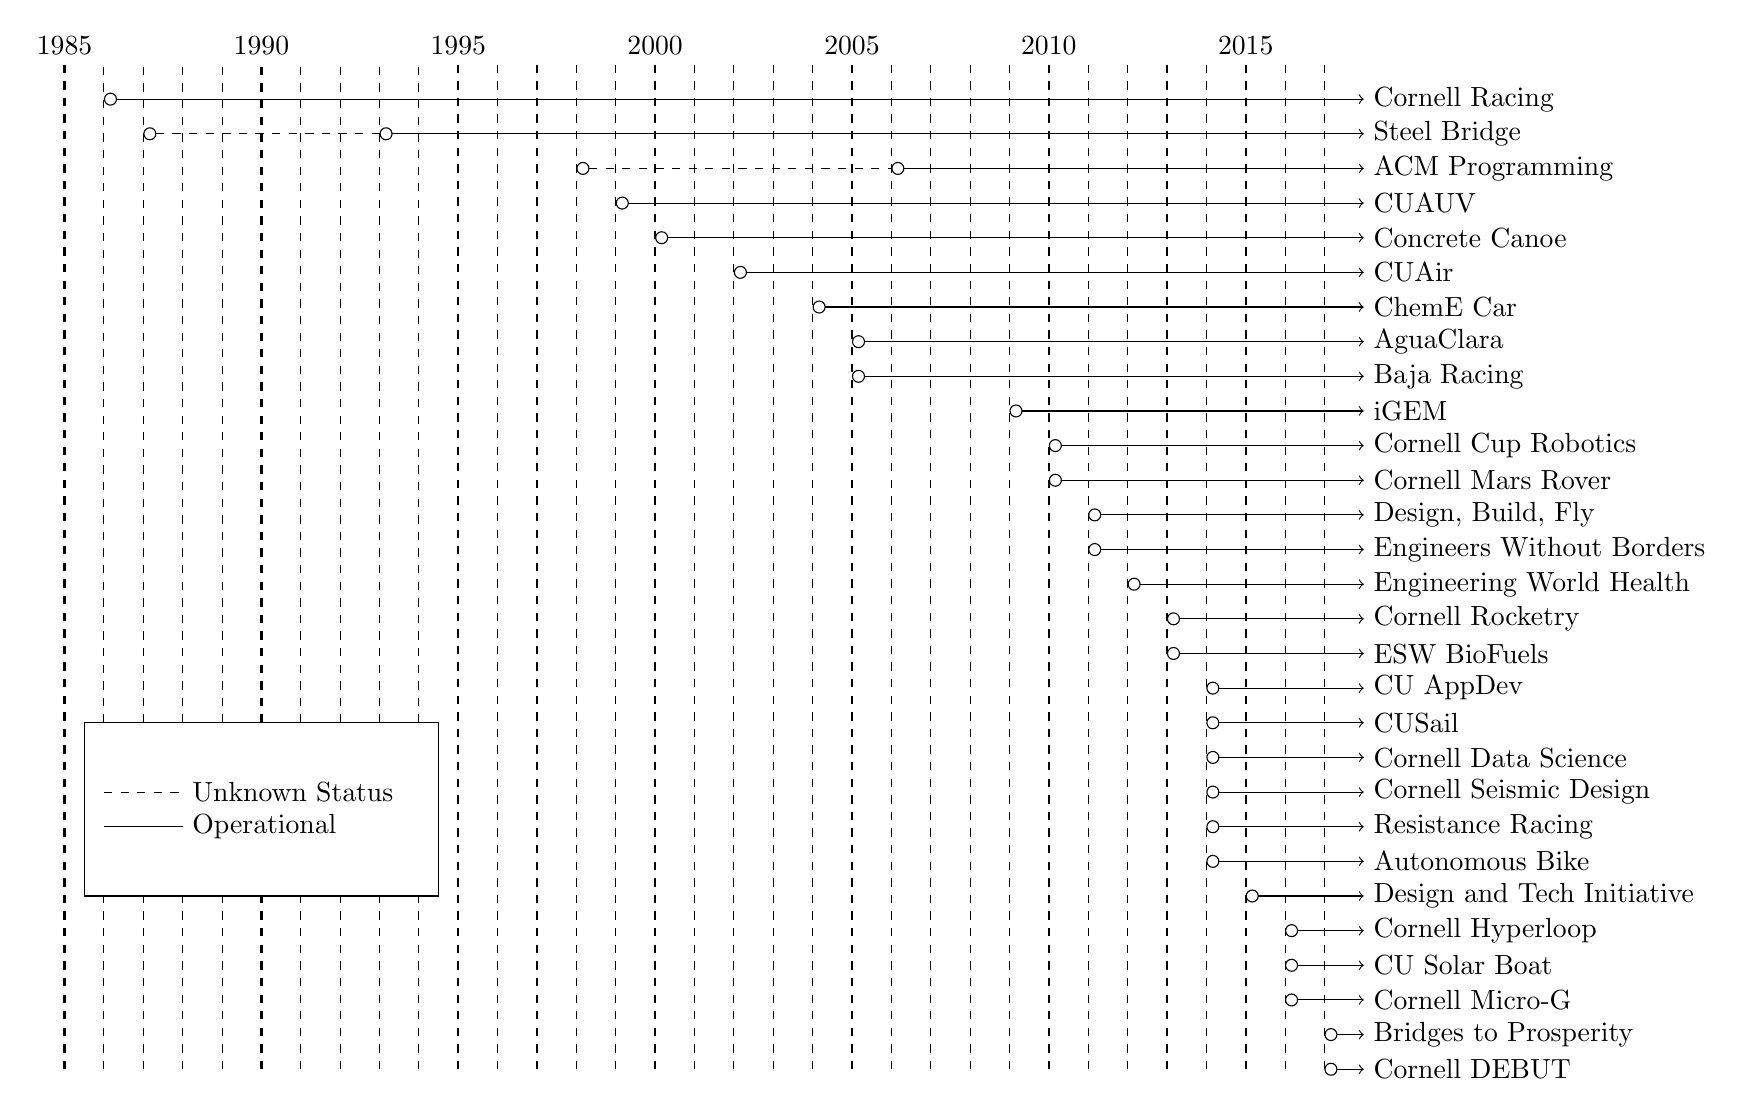
\begin{tikzpicture}[x=0.5cm, y=0.44cm]

\draw[dashed] (1, 8) -- (3, 8);
\node[right] at (3, 8) {Unknown Status};

\draw (1, 7) -- (3, 7);
\node[right] at (3, 7) {Operational};

\draw (0.5,5) -- (0.5,10) -- (9.5,10) -- (9.5,5) -- (0.5,5);


\node[above] at (0, 29) {1985};
\draw[dashed, thick] (0, 0) -- (0, 29);
\draw[dashed] (1, 0) -- (1, 5);
\draw[dashed] (1, 10) -- (1, 29);
\draw[dashed] (2, 0) -- (2, 5);
\draw[dashed] (2, 10) -- (2, 29);
\draw[dashed] (3, 0) -- (3, 5);
\draw[dashed] (3, 10) -- (3, 29);
\draw[dashed] (4, 0) -- (4, 5);
\draw[dashed] (4, 10) -- (4, 29);
\node[above] at (5, 29) {1990};
\draw[dashed, thick] (5, 0) -- (5, 5);
\draw[dashed, thick] (5, 10) -- (5, 29);
\draw[dashed] (6, 0) -- (6, 5);
\draw[dashed] (6, 10) -- (6, 29);
\draw[dashed] (7, 0) -- (7, 5);
\draw[dashed] (7, 10) -- (7, 29);
\draw[dashed] (8, 0) -- (8, 5);
\draw[dashed] (8, 10) -- (8, 29);
\draw[dashed] (9, 0) -- (9, 5);
\draw[dashed] (9, 10) -- (9, 29);
\node[above] at (10, 29) {1995};
\draw[dashed, thick] (10, 0) -- (10, 29);
\draw[dashed] (11, 0) -- (11, 29);
\draw[dashed] (12, 0) -- (12, 29);
\draw[dashed] (13, 0) -- (13, 29);
\draw[dashed] (14, 0) -- (14, 29);
\node[above] at (15, 29) {2000};
\draw[dashed, thick] (15, 0) -- (15, 29);
\draw[dashed] (16, 0) -- (16, 29);
\draw[dashed] (17, 0) -- (17, 29);
\draw[dashed] (18, 0) -- (18, 29);
\draw[dashed] (19, 0) -- (19, 29);
\node[above] at (20, 29) {2005};
\draw[dashed, thick] (20, 0) -- (20, 29);
\draw[dashed] (21, 0) -- (21, 29);
\draw[dashed] (22, 0) -- (22, 29);
\draw[dashed] (23, 0) -- (23, 29);
\draw[dashed] (24, 0) -- (24, 29);
\node[above] at (25, 29) {2010};
\draw[dashed, thick] (25, 0) -- (25, 29);
\draw[dashed] (26, 0) -- (26, 29);
\draw[dashed] (27, 0) -- (27, 29);
\draw[dashed] (28, 0) -- (28, 29);
\draw[dashed] (29, 0) -- (29, 29);
\node[above] at (30, 29) {2015};
\draw[dashed, thick] (30, 0) -- (30, 29);
\draw[dashed] (31, 0) -- (31, 29);
%\node[above] at (32, 29) {2017};
\draw[dashed] (32, 0) -- (32, 29);


% Cornell Racing: 1986
\node [right] at (33, 28) {Cornell Racing};
\draw[o->] (1, 28) -- (33, 28);

% Steel Bridge: 1987 -- 1993 - pres
\node [right] at (33, 27) {Steel Bridge};
\draw[dashed, o-] (2, 27) -- (8, 27);
\draw[o->] (8, 27) -- (33, 27);

% Cornell ACM Programming: 1998 -- 2006 - pres
\node [right] at (33, 26) {ACM Programming};
\draw[dashed, o-] (13, 26) -- (21, 26);
\draw[o->] (21, 26) -- (33, 26);

% CUAUV: 1999
\node [right] at (33, 25) {CUAUV};
\draw[o->] (14, 25) -- (33, 25);

% Concrete Canoe: 2000
\node [right] at (33, 24) {Concrete Canoe};
\draw[o->] (15, 24) -- (33, 24);

% CUAir: 2002
\node [right] at (33, 23) {CUAir};
\draw[o->] (17, 23) -- (33, 23);

% ChemE Car: 2004
\node [right] at (33, 22) {ChemE Car};
\draw[o->] (19, 22) -- (33, 22);

% AguaClara: 2005
\node [right] at (33, 21) {AguaClara};
\draw[o->] (20, 21) -- (33, 21);

% Baja Racing: 2005
\node [right] at (33, 20) {Baja Racing};
\draw[o->] (20, 20) -- (33, 20);

% iGEM: 2009
\node [right] at (33, 19) {iGEM};
\draw[o->] (24, 19) -- (33, 19);

% Cornell Cup Robotics: 2010
\node [right] at (33, 18) {Cornell Cup Robotics};
\draw[o->] (25, 18) -- (33, 18);

% Cornell Mars Rover: 2010
\node [right] at (33, 17) {Cornell Mars Rover};
\draw[o->] (25, 17) -- (33, 17);

% Design, Build, Fly: 2011
\node [right] at (33, 16) {Design, Build, Fly};
\draw[o->] (26, 16) -- (33, 16);

% Engineers Without Borders: 2011
\node [right] at (33, 15) {Engineers Without Borders};
\draw[o->] (26, 15) -- (33, 15);

% Engineering World Health: 2012
\node [right] at (33, 14) {Engineering World Health};
\draw[o->] (27, 14) -- (33, 14);

% Cornell Rocketry: 2013
\node [right] at (33, 13) {Cornell Rocketry};
\draw[o->] (28, 13) -- (33, 13);

% ESW Biofuels: 2013
\node [right] at (33, 12) {ESW BioFuels};
\draw[o->] (28, 12) -- (33, 12);

% CU AppDev: 2014
\node [right] at (33, 11) {CU AppDev};
\draw[o->] (29, 11) -- (33, 11);

% CUSail: 2014
\node [right] at (33, 10) {CUSail};
\draw[o->] (29, 10) -- (33, 10);

% Cornell Data Science: 2014
\node [right] at (33, 9) {Cornell Data Science};
\draw[o->] (29, 9) -- (33, 9);

% Cornell Seismic Design: 2014
\node [right] at (33, 8) {Cornell Seismic Design};
\draw[o->] (29, 8) -- (33, 8);

% Resistance Racing: 2014
\node [right] at (33, 7) {Resistance Racing};
\draw[o->] (29, 7) -- (33, 7);

% Autonomous Bike: 2014
\node [right] at (33, 6) {Autonomous Bike};
\draw[o->] (29, 6) -- (33, 6);

% Cornell Design and Tech Initiative: 2015
\node [right] at (33, 5) {Design and Tech Initiative};
\draw[o->] (30, 5) -- (33, 5);

% Cornell Hyperloop: 2016
\node [right] at (33, 4) {Cornell Hyperloop};
\draw[o->] (31, 4) -- (33, 4);

% CU Solar Boat: 2016
\node [right] at (33, 3) {CU Solar Boat};
\draw[o->] (31, 3) -- (33, 3);

% Cornell Micro-G: 2016
\node [right] at (33, 2) {Cornell Micro-G};
\draw[o->] (31, 2) -- (33, 2);

% Bridges to Prosperity: 2017
\node [right] at (33, 1) {Bridges to Prosperity};
\draw[o->] (32, 1) -- (33, 1);

% Cornell DEBUT: 2017
\node [right] at (33, 0) {Cornell DEBUT};
\draw[o->] (32, 0) -- (33, 0);

\end{tikzpicture}

%%% Local Variables:
%%% TeX-master: "report"
%%% End: %
    \caption{Timeline of current project teams at Cornell} %
    \label{fig:timeline} %
  \end{figure} %
\end{landscape} %
\noindent in number of project teams also tracks the explosion in number of enrolled Computer Science students (Figure~\ref{fig:teamcount}.
Given that a quarter of the project teams created in the last four years are primarily CS-related (CU AppDev, Cornell Data Science, and Design and Tech Initiative) and the majority of the rest have a CS component, the rapid increase in project teams and CS students could easily be related.

\begin{figure}
  \center
  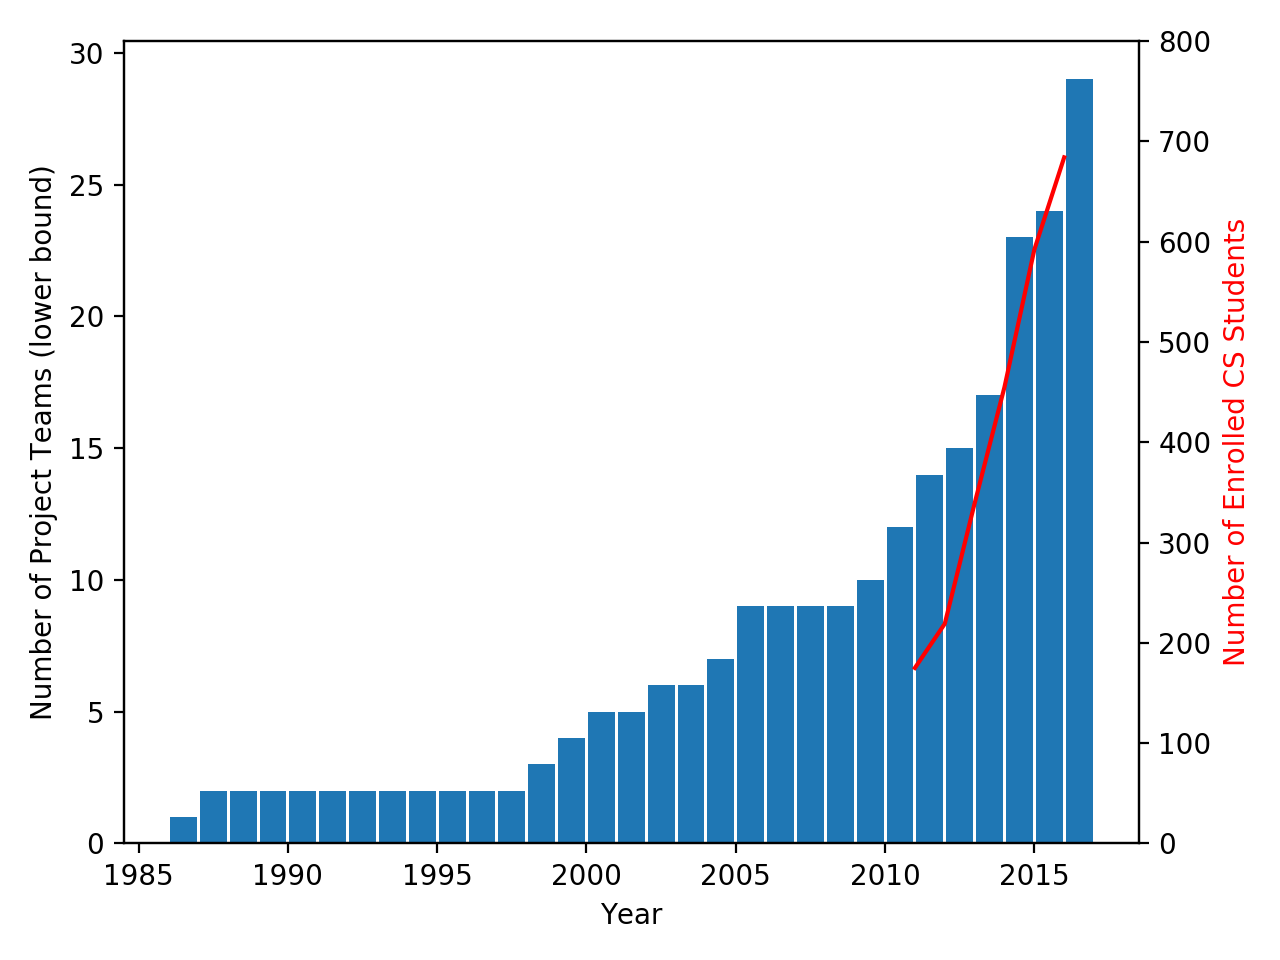
\includegraphics[width=0.7\textwidth]{teams-vs-cs}
  \caption{Number of project teams vs number of enrolled CS students~\cite{snabes_computer_2016}}
  \label{fig:teamcount}
\end{figure}


\section{Case Study: CUAUV}
\label{sec:cuauv}

Within the general trend of project team growth at Cornell, it is interesting to track the trajectory and history of individual project teams.
As a member of CUAUV, I wanted to learn more about my team's history and past success and challenges. The Cornell University Autonomous Underwater Vehicle (CUAUV) team participates in the yearly RoboSub competition, building an autonomous submarine to complete what is effectively an underwater obstacle course.


``The CUAUV team, as we know it today, was started by sophomores Serguei Vassilvitskii, Nidhi Kalra, Jack Chuang, and Walter Chang in September of 1999''
\cite{noauthor_cuauv_2003}. CUAUV was founded as BRAIN, the Big Red Artificial Intelligence Navigator, and competed in the year 2000 RoboSub competition, taking 2nd place (see Table~\ref{table:cuauv}).
Despite its youth, the team immediately picked up 40 students, a count which it has roughly continued to this day.

In 2003, BRAIN renamed itself to CUAUV.
That year also saw more major organizational changes to CUAUV, along with a more through documentation of them than would otherwise be possible, through Christopher Caufield's Master of Engineering project, ``Project management and systems engineeering practices of the Cornell University Autonomous Underwater Vehicle team: present and future''~\cite{caufield_project_2004}.
Caufield stated that ``the team is larger this year than ever before'', and better project management techniques were needed ``if the team was to work effectively at this size''.
This resulted in splitting the team up into subgroups of Software, Hull Propulsion and Infrastructure, and Sensors; descendents of which still exist today.
Caufield's project also saw the introduction of the Wiki to CUAUV, which allows for historical investigation of decisions made back to that year, including both design decisions for past subs and along with leadership and organizational changes.

\begin{figure}
  \centering

  \begin{tabular}{|c||c|c|c|c|c|c|c|c|c|c|c|c|c|c|c|c|c|c|c|c|}
    \hline
    \textbf{Placement} & \cellcolor{gray!50}2nd & 5th & \cellcolor{gray!50}2nd & \cellcolor{Goldenrod}1st & \cellcolor{gray!50}2nd & \textgreater 7th & \textgreater 7th & 4th & \textgreater 7th & \cellcolor{Goldenrod}1st & \cellcolor{Goldenrod}1st \\
    \hline
    \textbf{Year} & 2000 & 2001 & 2002 & 2003 & 2004 & 2005 & 2006 & 2007 & 2008 & 2009 & 2010\\
    \hline
  \end{tabular}
  \vspace{0.3cm}

  \begin{tabular}{|c||c|c|c|c|c|c|c|c|c|c|c|c|c|c|c|c|c|c|c|c|}
    \hline
    \textbf{Placement} & \cellcolor{gray!50}2nd & \cellcolor{Goldenrod}1st & \cellcolor{Goldenrod}1st & \cellcolor{Goldenrod}1st & \textgreater 8th & \cellcolor{RawSienna!75}3rd & \cellcolor{Goldenrod}1st\\
    \hline
    \textbf{Year} & 2011 & 2012 & 2013 & 2014 & 2015 & 2016 & 2017\\
    \hline
  \end{tabular}
  \captionof{table}{CUAUV historical placement~\cite{noauthor_robosub_2017}}
  \label{table:cuauv}
\end{figure}

\section{Conclusion}
\label{sec:conclusion}

From the 32 year veterans to the fresh-faced 1-year-olds, student-led project teams play a fundamental role in Cornell's success as an engineering school.
As of April 28, 2018, Cornell Engineering's website features a picture of the Cornell Mars Rover team~\cite{fleischman_rovers_2018} and the various web pages for prospective students all strongly advertise Cornell's 29 project teams, and for good reason -- anecdotally, project teams are a main reason that many students (myself included!) choose Cornell over other comparable schools.
Project teams are a central part of many Cornell engineering students' undergraduate careers, and can be a powerful force in the learning and success of students.
Cornell's project teams are clearly an establishment with staying power, and merit more study, not only into their history but also their impact on students and their long-term success.

\bibliographystyle{plainnat}
\bibliography{report}

\end{document}
